\documentclass[11pt,a4paper]{article}
\usepackage[T1]{fontenc}
\usepackage[utf8]{inputenc}
\usepackage{lmodern}
\usepackage{textcomp}
\usepackage[left=1.8cm,right=1.8cm,top=2.3cm,bottom=2.2cm,headheight=14pt,headsep=8pt]{geometry}
\usepackage{multicol}
\usepackage{xcolor}
\usepackage{fancyhdr}
\usepackage{graphicx}
\usepackage{array}
\usepackage{amsmath,amssymb}
\usepackage{setspace}
\usepackage{longtable}
\graphicspath{{../}}
\definecolor{ygreen}{RGB}{46,139,87}
\renewcommand{\normalsize}{\fontsize{10.9}{13.4}\selectfont}
\renewcommand{\familydefault}{\rmdefault}
\setlength{\parindent}{0pt}
\setlength{\columnsep}{0.8cm}
\setlength{\columnseprule}{0.4pt}
\setlength{\multicolsep}{3pt plus 1pt minus 1pt}
\renewcommand{\textsubscript}[1]{\ensuremath{_{\text{\fontsize{8}{8}\selectfont #1}}}}
\renewcommand{\textsuperscript}[1]{\ensuremath{^{\text{\fontsize{8}{8}\selectfont #1}}}}
\newcommand{\qn}[1]{\textbf{\fontsize{11.5}{13}\selectfont #1}}
\newcommand{\qsep}{\par\vspace{1pt}\noindent\rule{0pt}{0.4pt}\par\vspace{5pt}}
\newcommand{\fwrule}{\par\vspace{5pt}\noindent\rule{\linewidth}{1.4pt}\par\vspace{7pt}}
\newsavebox{\fitb}
\newcommand{\fitbox}[1]{\sbox{\fitb}{#1}\ifdim\wd\fitb>\linewidth\resizebox{\linewidth}{!}{\usebox{\fitb}}\else\usebox{\fitb}\fi}
\newcommand{\diqqat}[1]{\par\smallskip\noindent\textbf{Diqqat!} #1\par\medskip}
\newcommand{\javob}{\par\smallskip\noindent\textbf{Javob:} \rule[-2pt]{7.5cm}{0.4pt}\par\smallskip\noindent\textbf{Diqqat!} Javobingizni javoblar varaqasiga ko`chirib yozing.\par\medskip}
\pagestyle{fancy}
\fancyhf{}
\renewcommand{\headrulewidth}{0.4pt}
\fancyhead[L]{\textit{Milliy sertifikat 2026. Kimyo}}
\fancyhead[R]{7-variant}
\fancyfoot[L]{\fontsize{8}{9}\selectfont \textcopyright{} Colba maktabi, 2026}
\fancyfoot[C]{\thepage}
\fancypagestyle{first}{\fancyhf{}\renewcommand{\headrulewidth}{0pt}\fancyfoot[L]{\fontsize{8}{9}\selectfont \textcopyright{} Colba maktabi, 2026}\fancyfoot[C]{\thepage}}
\begin{document}
\normalsize
\thispagestyle{first}
\noindent\fcolorbox{ygreen}{white}{\parbox{\dimexpr\linewidth-2\fboxsep-2\fboxrule\relax}{%
\textbf{\fontsize{13}{15}\selectfont Nazorat testi}\ \textit{\fontsize{10}{12}\selectfont $\cdot$ Aralash test $\cdot$ 7-variant}\hfill
\begin{tabular}[t]{@{}r@{}}\textit{Milliy sertifikat 2026. Kimyo}\\ \textbf{\textit{\fontsize{8}{9}\selectfont Vaqt:}} \textit{\fontsize{10}{12}\selectfont 180 daqiqa}\end{tabular}}}
\par\medskip
\noindent\textit{Davriy jadvaldan foydalanish mumkin.}
\par\medskip
\begin{multicols}{2}
\noindent\qn{1.} 1 mol CO\textsubscript{2} tarkibida necha mol atom bor?

\noindent A)~\textsl{3} \hfill B)~\textsl{2} \hfill C)~\textsl{4} \hfill D)~\textsl{1}\par
\qsep
\noindent\qn{2.} pH = 9 bo`lgan eritmada gidroksid ionlari konsentratsiyasi 10\textsuperscript{$-$x} mol/l ga teng. x \textbf{ni aniqlang.}

\noindent A)~\textsl{9} \hfill B)~\textsl{5} \hfill C)~\textsl{6} \hfill D)~\textsl{8}\par
\qsep
\noindent\qn{3.} Tuzning eruvchanligi yuqori haroratda 150 g, past haroratda 40 g (100 g suvda). Yuqori haroratda to`yingan 500 g eritma past haroratgacha sovitilsa, necha gramm tuz cho`kmaga tushadi?

\noindent A)~\textsl{300} \hfill B)~\textsl{80} \hfill C)~\textsl{220} \hfill D)~\textsl{440}\par
\qsep
\noindent\qn{4.} Zichligi 1,11 g/ml bo`lgan 10\% li NaOH eritmasining molyar \textbf{konsentratsiyasini (mol/l) aniqlang.}

\noindent A)~\textsl{2,78} \hfill B)~\textsl{0,28} \hfill C)~\textsl{5,55} \hfill D)~\textsl{2,5}\par
\qsep
\noindent\qn{5.} Gazlar aralashmasi tarkibi jadvalda berilgan (n.sh.):
\begin{center}
\renewcommand{\arraystretch}{1.15}
\fitbox{\begin{tabular}{|c|c|}\hline
\textbf{Gaz} & \textbf{Hajmi, l} \\ \hline
CO\textsubscript{2} & 1 \\ \hline
N\textsubscript{2} & 2 \\ \hline
SO\textsubscript{2} & 3 \\ \hline
\end{tabular}}
\end{center}
Aralashmaning havoga nisbatan \textbf{zichligini aniqlang} (M(havo) = 29 g/mol).

\noindent A)~\textsl{1,68} \hfill B)~\textsl{3,36} \hfill C)~\textsl{0,84} \hfill D)~\textsl{48,67}\par
\qsep
\noindent\qn{6.} Metall oksidida kislorodning massa ulushi 22,22\%. Metallning ekvivalent \textbf{massasini (g/mol) aniqlang.}

\noindent A)~\textsl{56} \hfill B)~\textsl{14} \hfill C)~\textsl{28} \hfill D)~\textsl{42}\par
\qsep
\noindent\qn{7.} Jadvalda nuklidlarning proton soni (\textit{Z}) va massa soni (A) berilgan:
\begin{center}
\renewcommand{\arraystretch}{1.15}
\fitbox{\begin{tabular}{|c|c|c|}\hline
\textbf{Nuklid} & \textbf{\textit{Z}} & \textbf{A} \\ \hline
\textit{X} & 20 & 40 \\ \hline
\textit{Y} & 20 & 42 \\ \hline
T & 21 & 40 \\ \hline
\textit{U} & 21 & 41 \\ \hline
\textit{V} & 20 & 42 \\ \hline
\end{tabular}}
\end{center}
\textit{X} nuklidning nechta izobari jadvalda keltirilgan?

\noindent A)~\textsl{2} \hfill B)~\textsl{3} \hfill C)~\textsl{1} \hfill D)~\textsl{4}\par
\qsep
\noindent\qn{8.} Quyidagi tuzlarning qaysilari suvli eritmasi ishqoriy muhitga ega? 1) CH\textsubscript{3}COONa; 2) FeCl\textsubscript{3}; 3) Al\textsubscript{2}(SO\textsubscript{4})\textsubscript{3}; 4) Na\textsubscript{2}CO\textsubscript{3}

\noindent A)~\textsl{1, 3} \hfill B)~\textsl{3} \hfill C)~\textsl{1} \hfill D)~\textsl{1, 4}\par
\qsep
\noindent\qn{9.} Hajmi 5 l bo`lgan idishda A modda miqdori 30 s davomida 3 mol ga kamaydi. Reaksiyaning o`rtacha tezligini (mol/(l$\cdot$s)) \textbf{toping.}

\noindent A)~\textsl{0,1} \hfill B)~\textsl{0,6} \hfill C)~\textsl{0,02} \hfill D)~\textsl{0,5}\par
\qsep
\noindent\qn{10.} VA guruh elementlarining vodorodli birikmalari qaynash haroratlari grafikda berilgan.
\begin{center}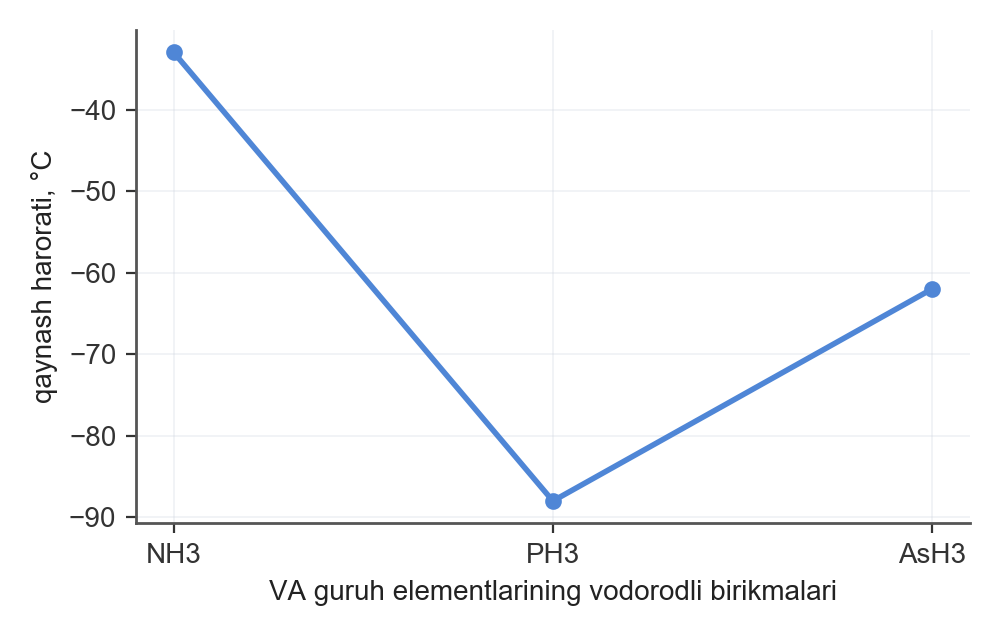
\includegraphics[width=0.86\linewidth]{rasmlar/gen/hy2_v07_0.png}\end{center}
Qaysi birikmaning qaynash harorati qonuniyatdan keskin farq qiladi?

\noindent A)~\textsl{NH\textsubscript{3}} \hfill B)~\textsl{PH\textsubscript{3}} \hfill C)~\textsl{AsH\textsubscript{3}}\par
\qsep
\noindent\qn{11.} Rux (\textit{Z} = 30) atomining tashqi energetik pog`onasidagi elektronlar \textbf{sonini aniqlang.}

\noindent A)~\textsl{3} \hfill B)~\textsl{1} \hfill C)~\textsl{4} \hfill D)~\textsl{2}\par
\qsep
\noindent\qn{12.} A + B $\to$ mahsulot reaksiyada v = k$\cdot$[A]\textsuperscript{2}$\cdot$[B]\textsuperscript{2}. Idish hajmi 2 marta kamaytirilsa (T = const), reaksiya tezligi necha marta o`zgaradi?

\noindent A)~\textsl{4} \hfill B)~\textsl{2} \hfill C)~\textsl{16} \hfill D)~\textsl{32}\par
\qsep
\noindent\qn{13.} Rasmda tasvirlangan A elementi haqida qaysi fikr to`g`ri?
\begin{center}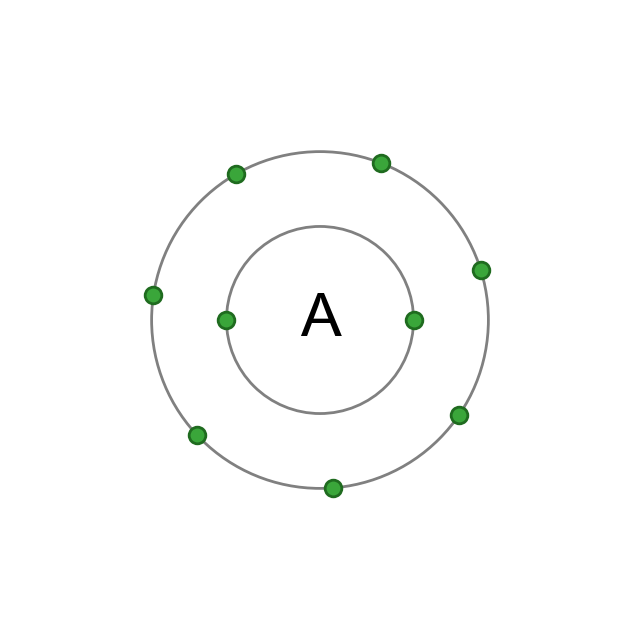
\includegraphics[width=0.86\linewidth]{rasmlar/gen/atom_9_16432.png}\end{center}
\noindent A)~\textsl{Metall, oksidi asosli xossali}\par
\noindent B)~\textsl{Metall, vodorodli birikma hosil qilmaydi}\par
\noindent C)~\textsl{Inert gaz, birikmalar hosil qilmaydi}\par
\noindent D)~\textsl{Metallmas, oksidi kislotali xossali}\par
\qsep
\noindent\qn{14.} 3,1 g fosfor yondirilib, hosil bo`lgan oksid suvda eritildi (ortofosfat kislota), so`ng 0,3 mol NaOH qo`shildi. Hosil bo`lgan Na\textsubscript{3}PO\textsubscript{4} \textbf{massasini (g) aniqlang.}

\noindent A)~\textsl{32,8} \hfill B)~\textsl{16,4} \hfill C)~\textsl{8,2} \hfill D)~\textsl{12}\par
\qsep
\noindent\qn{15.} NaBr + AgNO\textsubscript{3} $\to$ AgBr + NaNO\textsubscript{3} reaksiyasida 51,5 g NaBr ishtirok etdi. AgBr \textbf{miqdorini (mol) toping.}

\noindent A)~\textsl{1} \hfill B)~\textsl{0,25} \hfill C)~\textsl{0,75} \hfill D)~\textsl{0,5}\par
\qsep
\noindent\qn{16.} Ishqoriy metallar haqida qaysi fikrlar to`g`ri? 1) Natriy yonganda Na\textsubscript{2}O\textsubscript{2} hosil bo`ladi; 2) Natriy kerosin ostida saqlanadi; 3) Natriyning olinishi suyuqlanma NaCl elektrolizi bilan; 4) Ishqoriy metallar tabiatda erkin holda uchraydi

\noindent A)~\textsl{2, 4} \hfill B)~\textsl{2, 3} \hfill C)~\textsl{1, 3, 4} \hfill D)~\textsl{1, 2, 3}\par
\qsep
\noindent\qn{17.} Alyuminiy va magniy dan iborat 5,1 g aralashma mo`l xlorid kislotada eritilganda 5,6 l (n.sh.) vodorod ajraldi. Aralashmadagi alyuminiyning massa \textbf{ulushini (\%) aniqlang.}

\noindent A)~\textsl{52,9} \hfill B)~\textsl{47,1} \hfill C)~\textsl{26,5} \hfill D)~\textsl{2,7}\par
\qsep
\noindent\qn{18.} D-metallar va ularning birikmalari haqida qaysi fikrlar to`g`ri? 1) Cu(OH)\textsubscript{2} qizdirilganda CuO ga parchalanadi; 2) Fe(OH)\textsubscript{2} havoda qo`ng`ir rangga o`tadi; 3) Cr\textsubscript{2}O\textsubscript{3} asosli oksid; 4) Mis suyultirilgan HCl bilan reaksiyaga kirishadi

\noindent A)~\textsl{1, 2} \hfill B)~\textsl{4} \hfill C)~\textsl{1, 2, 3} \hfill D)~\textsl{1, 3, 4}\par
\qsep
\noindent\qn{19.} 0,1 mol Ca(HCO\textsubscript{3})\textsubscript{2} tutgan suv qaynatilganda hosil bo`lgan CaCO\textsubscript{3} cho`kma massasini (g)  \textbf{ni toping.}

\noindent A)~\textsl{20} \hfill B)~\textsl{10} \hfill C)~\textsl{5} \hfill D)~\textsl{15}\par
\qsep
\noindent\qn{20.} CH\textsubscript{3}--C(CH\textsubscript{3})\textsubscript{2}--CH\textsubscript{2}--CH\textsubscript{3} birikmaning sistematik nomi qaysi qatorda to`g`ri keltirilgan?

\noindent\begin{tabular}{@{}p{0.47\linewidth}@{}p{0.47\linewidth}@{}}
A)~\textsl{2-metilpentan} & B)~\textsl{3,3-dimetilbutan} \\
C)~\textsl{2,2-dimetilpropan} & D)~\textsl{2,2-dimetilbutan} \\
\end{tabular}\par
\qsep
\noindent\qn{21.} Etilen va asetilendan iborat 5,4 g aralashmani to`liq gidrogenlash uchun sarflanadigan vodorod \textbf{hajmini (l, n.sh.) aniqlang.} Aralashmadagi etilen va asetilenning mol nisbati 1 : 1.

\noindent A)~\textsl{13,44} \hfill B)~\textsl{6,72} \hfill C)~\textsl{3,36} \hfill D)~\textsl{4,48}\par
\qsep
\noindent\qn{22.} Reaksiya tenglamasi: 2C\textsubscript{6}H\textsubscript{6} + 15O\textsubscript{2} $\to$ 12CO\textsubscript{2} + 6H\textsubscript{2}O. Reaksiyaga 32 g O\textsubscript{2} kirishdi. CO\textsubscript{2} \textbf{hajmini (l, n.sh.) hisoblang.}

\noindent A)~\textsl{28} \hfill B)~\textsl{35,84} \hfill C)~\textsl{8,96} \hfill D)~\textsl{17,92}\par
\qsep
\noindent\qn{23.} CH\textsubscript{3}CHO + Ag\textsubscript{2}O (NH\textsubscript{3}) reaksiyasi natijasida qaysi organik modda hosil bo`ladi?

\noindent\begin{tabular}{@{}p{0.47\linewidth}@{}p{0.47\linewidth}@{}}
A)~\textsl{etilatsetat} & B)~\textsl{sirka kislota} \\
C)~\textsl{metan} & D)~\textsl{sirka aldegid} \\
\end{tabular}\par
\qsep
\noindent\qn{24.} Aldegid va ketonlar haqida qaysi fikrlar to`g`ri? 1) Formalin --- formaldegidning 40\% li eritmasi; 2) Sirka aldegid Kucherov reaksiyasi bilan olinadi; 3) Aseton suvda erimaydi; 4) Formaldegid gaz holatda, suvda yaxshi eriydi

\noindent A)~\textsl{1, 3, 4} \hfill B)~\textsl{1, 2, 4} \hfill C)~\textsl{1, 4} \hfill D)~\textsl{2, 3, 4}\par
\qsep
\noindent\qn{25.} Karbon kislotalar haqida qaysi fikrlar to`g`ri? 1) Sirka kislota karbonatlar bilan CO\textsubscript{2} ajratadi; 2) Sirka angidrid ikki molekula sirka kislotadan suv chiqib hosil bo`ladi; 3) Benzoy kislota Na\textsubscript{2}CO\textsubscript{3} bilan reaksiyaga kirishmaydi; 4) Karboksil guruh karbonil va gidroksil guruhlardan iborat

\noindent A)~\textsl{3, 4} \hfill B)~\textsl{2, 3} \hfill C)~\textsl{1, 2, 4} \hfill D)~\textsl{1, 3}\par
\qsep
\noindent\qn{26.} 88 g CH\textsubscript{3}COOC\textsubscript{2}H\textsubscript{5} dan quyidagi ikki bosqichda C\textsubscript{2}H\textsubscript{4} olinadi: 1) CH\textsubscript{3}COOC\textsubscript{2}H\textsubscript{5} + H\textsubscript{2}O $\to$ CH\textsubscript{3}COOH + C\textsubscript{2}H\textsubscript{5}OH (unum 75\%); 2) C\textsubscript{2}H\textsubscript{5}OH $\to$ C\textsubscript{2}H\textsubscript{4} + H\textsubscript{2}O (unum 50\%). Oxirgi mahsulot C\textsubscript{2}H\textsubscript{4} ning \textbf{hajmini (l, n.sh.) toping.}

\noindent A)~\textsl{11,2} \hfill B)~\textsl{16,8} \hfill C)~\textsl{8,4} \hfill D)~\textsl{22,4}\par
\qsep
\noindent\qn{27.} 68,4 g maltoza to`liq gidrolizlanib, hosil bo`lgan mahsulot Ag\textsubscript{2}O ning ammiakli eritmasi bilan oksidlandi. Ajralgan kumush \textbf{massasini (g) aniqlang.}

\noindent A)~\textsl{43,2} \hfill B)~\textsl{172,8} \hfill C)~\textsl{86,4} \hfill D)~\textsl{21,6}\par
\qsep
\noindent\qn{28.} 61,5 g C\textsubscript{6}H\textsubscript{5}NO\textsubscript{2} dan quyidagi ikki bosqichda C\textsubscript{6}H\textsubscript{5}NH\textsubscript{3}Cl olinadi: 1) C\textsubscript{6}H\textsubscript{5}NO\textsubscript{2} + 3H\textsubscript{2} $\to$ C\textsubscript{6}H\textsubscript{5}NH\textsubscript{2} + 2H\textsubscript{2}O (unum 80\%); 2) C\textsubscript{6}H\textsubscript{5}NH\textsubscript{2} + HCl $\to$ C\textsubscript{6}H\textsubscript{5}NH\textsubscript{3}Cl (unum 75\%). Oxirgi mahsulot C\textsubscript{6}H\textsubscript{5}NH\textsubscript{3}Cl ning \textbf{massasini (g) toping.}

\noindent A)~\textsl{48,56} \hfill B)~\textsl{38,85} \hfill C)~\textsl{51,8} \hfill D)~\textsl{64,75}\par
\qsep
\noindent\qn{29.} Vinilxlorid monomeridan olingan polimerning molyar massasi 62500 g/mol. Polimerlanish \textbf{darajasini aniqlang.}

\noindent A)~\textsl{1000} \hfill B)~\textsl{2000} \hfill C)~\textsl{500} \hfill D)~\textsl{1010}\par
\qsep
\noindent\qn{30.} Rasmdagi asbobda oxirgi idishga NaOH eritmasi solingan. Uning vazifasi nima?
\begin{center}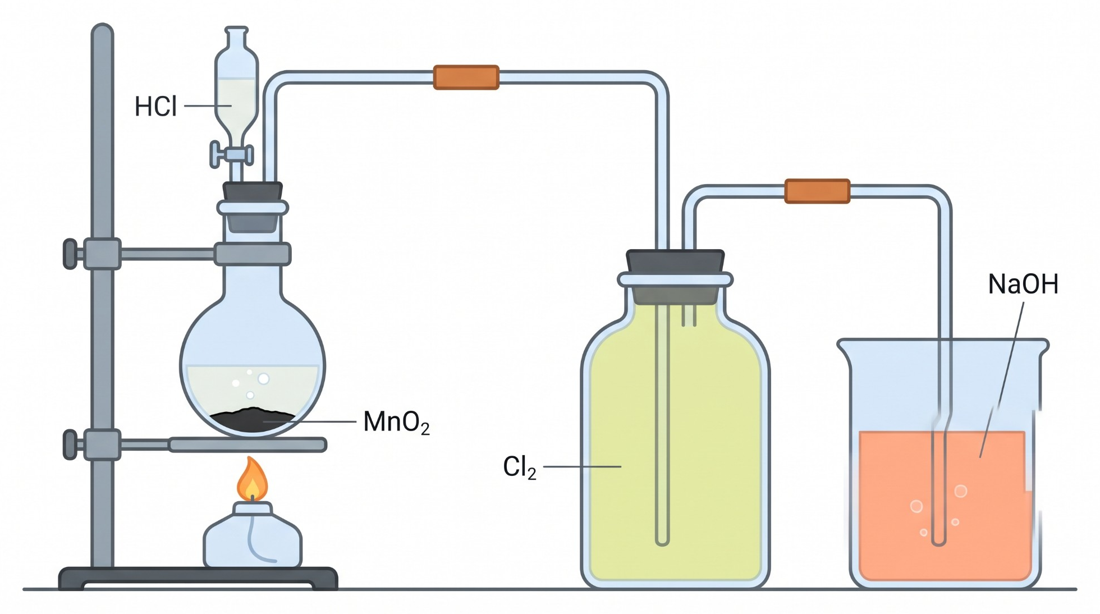
\includegraphics[width=0.86\linewidth]{rasmlar/darslik/d_xlor.png}\end{center}
\noindent A)~\textsl{xlorni suvda eritish}\par
\noindent B)~\textsl{ortiqcha xlorni yutib, atrof-muhitni zaharlanishdan saqlash}\par
\noindent C)~\textsl{xlorni quritish}\par
\noindent D)~\textsl{reaksiyani tezlashtirish}\par
\qsep
\noindent\qn{31.} I\textsuperscript{$-$} ionini aniqlash uchun qaysi reagent mos va qanday belgi kuzatiladi?
\noindent A)~\textsl{AgNO\textsubscript{3}: sariq cho`kma (AgI), HNO\textsubscript{3} da erimaydi}\par
\noindent B)~\textsl{NaOH: qo`ng`ir cho`kma (Fe(OH)\textsubscript{3})}\par
\noindent C)~\textsl{HCl: rangsiz gaz (CO\textsubscript{2}) ajraladi}\par
\noindent D)~\textsl{AgNO\textsubscript{3}: sariq cho`kma (Ag\textsubscript{3}PO\textsubscript{4}), HNO\textsubscript{3} da eriydi}\par
\qsep
\noindent\qn{32.} Uch probirkada (\textit{X}, \textit{Y}, \textit{Z}) Na\textsubscript{2}SO\textsubscript{4}, K\textsubscript{2}CO\textsubscript{3}, NH\textsubscript{4}Cl eritmalari bor (tartibsiz). Ularga HCl va NaOH ta'sir ettirildi. Kuzatuvlar jadvalda:
\begin{center}
\renewcommand{\arraystretch}{1.15}
\fitbox{\begin{tabular}{|c|c|c|}\hline
\textbf{Probirka} & \textbf{HCl qo`shilganda} & \textbf{NaOH qo`shib qizdirilganda} \\ \hline
\textit{X} & gaz ajraladi & o`zgarish yo`q \\ \hline
\textit{Y} & o`zgarish yo`q & o`tkir hidli gaz ajraladi \\ \hline
\textit{Z} & o`zgarish yo`q & o`zgarish yo`q \\ \hline
\end{tabular}}
\end{center}
\textit{X}, \textit{Y}, \textit{Z} probirkalardagi \textbf{moddalarni aniqlang.}
\noindent A)~\textsl{\textit{X} -- NH\textsubscript{4}Cl, \textit{Y} -- Na\textsubscript{2}SO\textsubscript{4}, \textit{Z} -- K\textsubscript{2}CO\textsubscript{3}}\par
\noindent B)~\textsl{\textit{X} -- Na\textsubscript{2}SO\textsubscript{4}, \textit{Y} -- NH\textsubscript{4}Cl, \textit{Z} -- K\textsubscript{2}CO\textsubscript{3}}\par
\noindent C)~\textsl{\textit{X} -- NH\textsubscript{4}Cl, \textit{Y} -- K\textsubscript{2}CO\textsubscript{3}, \textit{Z} -- Na\textsubscript{2}SO\textsubscript{4}}\par
\noindent D)~\textsl{\textit{X} -- K\textsubscript{2}CO\textsubscript{3}, \textit{Y} -- NH\textsubscript{4}Cl, \textit{Z} -- Na\textsubscript{2}SO\textsubscript{4}   ---}\par
\qsep
\end{multicols}
\medskip
\noindent\setlength{\fboxsep}{0pt}\fbox{\begin{tabular}{p{0.74\linewidth}|p{0.2\linewidth}}
\parbox[t]{0.72\linewidth}{\vspace{3pt}\textbf{Topshiriqlar (33--35) va javob variant (A--F)larini o`zaro to`g`ri moslashtiring.} NaHCO\textsubscript{3} va KHCO\textsubscript{3} dan iborat 36,8 g aralashma mo`l xlorid kislota bilan to`liq reaksiyaga kirishdi.
\vspace{3pt}} & \parbox[t]{0.19\linewidth}{\vspace{3pt}A~\textsl{32}\\[3pt]
B~\textsl{8,96}\\[3pt]
C~\textsl{40}\\[3pt]
D~\textsl{116,8}\\[3pt]
E~\textsl{146}\\[3pt]
F~\textsl{7,17}}\\ \hline
\parbox[t]{0.72\linewidth}{\vspace{2pt}\textbf{33. Ajralgan gaz hajmini (l, n.sh.) aniqlang.}\vspace{2pt}} & \\ \hline
\parbox[t]{0.72\linewidth}{\vspace{2pt}\textbf{34. Aralashmani to`liq eritish uchun sarflangan 10\% li HCl eritmasining massasini (g) aniqlang (M(HCl) = 36,5 g/mol).}\vspace{2pt}} & \\ \hline
\parbox[t]{0.72\linewidth}{\vspace{2pt}\textbf{35. Ajralgan gaz mo`l Ca(OH)\textsubscript{2} eritmasidan o`tkazilganda hosil bo`lgan cho`kma massasini (g) aniqlang.}\vspace{2pt}} & 
\end{tabular}}
\par\bigskip
\noindent\qn{36.} KMnO\textsubscript{4} + KI + H\textsubscript{2}SO\textsubscript{4} $\to$ MnSO\textsubscript{4} + I\textsubscript{2} + K\textsubscript{2}SO\textsubscript{4} + H\textsubscript{2}O reaksiya tenglamasini elektron balans usulida tenglang va barcha koeffitsiyentlar \textbf{yig`indisini aniqlang.}
\javob\qsep
\noindent\qn{37.} AgNO\textsubscript{3} eritmasi inert elektrodlar yordamida 2 A tok kuchi bilan 965 s elektroliz qilindi. Anodda ajralgan O\textsubscript{2} hajmi (l, n.sh.) \textbf{ni toping.}
\javob\qsep
\noindent\qn{38.} 47 g Cu(NO\textsubscript{3})\textsubscript{2} to`liq parchalanguncha qizdirildi. Qattiq qoldiq \textbf{massasini (g) aniqlang.}
\javob\qsep
\noindent\qn{39.} 12 g sirka kislotani neytrallash uchun 10\% li NaOH eritmasidan necha gramm kerak?
\javob\qsep
\noindent\qn{40.} 12,3 g nitrobenzol anilinga qaytarildi (unum 80\%), hosil bo`lgan anilin mo`l bromli suv bilan reaksiyaga kirishdi (unum 80\%). Hosil bo`lgan 2,4,6-tribromanilin (M = 330 g/mol) \textbf{massasini (g) toping.}
\javob\qsep
\par\bigskip\begin{center}\textbf{\fontsize{13}{15}\selectfont YOZMA ISH}\end{center}
\noindent\qn{41.} \textbf{Topshiriqni bajarish jarayonida barcha reaksiya tenglamalarini yozing. Miqdoriy va arifmetik hisoblashlarni (unga asos bo`lgan usul yoki formulani ko`rsatgan holda) uzviy ketma-ketlikda bajaring.}\par\smallskip
29,25 g NaCl 300 g suvda eritildi. Hosil bo`lgan eritma inert elektrodlar yordamida 20 A tok kuchi bilan 965 s davomida elektroliz qilindi.\par
\noindent 1)Elektroliz tenglamasini yozing. Katodda va anodda ajralgan gazlarning hajmini (l, n.sh.) hisoblang (F = 96500 C/mol).\par
\noindent 2)Elektroliz qilingan NaCl ning massasini (g) toping. Elektroliz davomida o`tgan zaryadni (C) ham hisoblang.\par
\noindent 3)Elektroliz tugagach eritmadagi NaOH va qolgan NaCl ning massa ulushlarini (\%) aniqlang.\par
\noindent 4)Anodda ajralgan gaz mo`l KI eritmasidan o`tkazildi. Ajralgan yodning massasini (g) hisoblang (reaksiya tenglamasini yozing). Neytrallash uchun sarflangan HCl miqdorini (mol) ham toping.\par
\noindent 5)Elektroliz tugagan eritmani to`liq neytrallash uchun 10\% li HCl eritmasidan necha gramm kerak? Elektroliz tugagan eritmadan CO\textsubscript{2} o`rta tuz (karbonat) hosil bo`lguncha yuttirilsa, hosil bo`ladigan karbonat massasini (g) ham hisoblang.\par
\diqqat{Mazkur topshiriq kengaytirilgan javobni talab etib, uning yechilish usuli va shu usul asosidagi barcha hisoblash amallari javoblar varaqasida aks etishi lozim.}\qsep
\noindent\qn{42.} Quyidagi o`zgarishlar zanjirida \textit{X}, \textit{Y}, \textit{Z} noma'lum organik moddalar:\par
\[\setlength{\fboxsep}{0pt}\text{C\textsubscript{2}H\textsubscript{2}}\xrightarrow{\text{H\textsubscript{2}O, Hg\textsuperscript{2+}}}\text{\textit{X}}\xrightarrow{\text{Ag\textsubscript{2}O, NH\textsubscript{3}}}\text{\textit{Y}}\xrightarrow{\text{Cl\textsubscript{2}, P}}\text{ClCH\textsubscript{2}COOH}\]
\noindent 1)C\textsubscript{2}H\textsubscript{2} $\to$ \textit{X} : reaksiya tenglamasini yozing; hosil bo`lgan moddani nomlang.\par
\noindent 2)\textit{X} $\to$ \textit{Y} : reaksiya tenglamasini yozing; hosil bo`lgan moddani nomlang.\par
\noindent 3)\textit{Y} $\to$ ClCH\textsubscript{2}COOH : reaksiya tenglamasini yozing; hosil bo`lgan moddani nomlang.\par
\diqqat{Mazkur topshiriq kengaytirilgan javobni talab etib, uning yechilish usuli va shu usul asosidagi barcha hisoblash amallari javoblar varaqasida aks etishi lozim.}\qsep
\noindent\qn{43.} \textbf{Topshiriqni bajarish jarayonida barcha reaksiya tenglamalarini yozing. Miqdoriy va arifmetik hisoblashlarni (unga asos bo`lgan usul yoki formulani ko`rsatgan holda) uzviy ketma-ketlikda bajaring.}\par\smallskip
11,2 g temir mo`l xlorda yondirildi. Hosil bo`lgan tuz suvda eritilib, avval ishqor bilan, so`ng boshqa porsiyasi KI eritmasi bilan ta'sirlashtirildi.\par
\noindent 1)Reaksiya tenglamasini yozing. Sarflangan xlor hajmini (l, n.sh.) va hosil bo`lgan tuz massasini (g) toping. Hosil bo`lgan FeCl\textsubscript{3} miqdorini (mol) ham toping.\par
\noindent 2)Tuz eritmasiga mo`l NaOH qo`shilganda hosil bo`lgan cho`kma massasini (g) aniqlang.\par
\noindent 3)Cho`kma qizdirilganda hosil bo`ladigan oksid massasini (g) hisoblang.\par
\noindent 4)Tuzning shunday miqdoriga mo`l KI qo`shilganda ajraladigan yod massasini (g) toping (2FeCl\textsubscript{3} + 2KI $\to$ 2FeCl\textsubscript{2} + 2KCl + I\textsubscript{2}).\par
\noindent 5)Hosil bo`lgan FeCl\textsubscript{3} eritmasiga temir qo`shilib FeCl\textsubscript{2} hosil qilindi (2FeCl\textsubscript{3} + Fe $\to$ 3FeCl\textsubscript{2}). Sarflangan temir massasini (g) toping.\par
\diqqat{Mazkur topshiriq kengaytirilgan javobni talab etib, uning yechilish usuli va shu usul asosidagi barcha hisoblash amallari javoblar varaqasida aks etishi lozim.}\qsep
\newpage
\noindent\textbf{\fontsize{13}{15}\selectfont Nazorat testi}\ \textit{$\cdot$ 7-variant}\hfill \textbf{Javoblar kaliti}\par\smallskip\hrule\smallskip
\textit{Faqat o`qituvchi uchun.}\par\medskip
\noindent\textbf{1--32-savollar}\par\smallskip
\noindent\begin{tabular}{|c|c|c|c|c|c|c|c|c|c|c|c|c|c|c|c|}\hline
\textbf{1} & \textbf{2} & \textbf{3} & \textbf{4} & \textbf{5} & \textbf{6} & \textbf{7} & \textbf{8} & \textbf{9} & \textbf{10} & \textbf{11} & \textbf{12} & \textbf{13} & \textbf{14} & \textbf{15} & \textbf{16}\\\hline
\textsl{A} & \textsl{B} & \textsl{C} & \textsl{A} & \textsl{A} & \textsl{C} & \textsl{C} & \textsl{D} & \textsl{C} & \textsl{A} & \textsl{D} & \textsl{C} & \textsl{D} & \textsl{B} & \textsl{D} & \textsl{D}\\\hline
\textbf{17} & \textbf{18} & \textbf{19} & \textbf{20} & \textbf{21} & \textbf{22} & \textbf{23} & \textbf{24} & \textbf{25} & \textbf{26} & \textbf{27} & \textbf{28} & \textbf{29} & \textbf{30} & \textbf{31} & \textbf{32}\\\hline
\textsl{A} & \textsl{A} & \textsl{B} & \textsl{D} & \textsl{B} & \textsl{D} & \textsl{B} & \textsl{B} & \textsl{C} & \textsl{C} & \textsl{C} & \textsl{B} & \textsl{A} & \textsl{B} & \textsl{A} & \textsl{D}\\\hline
\end{tabular}\par\medskip
\noindent\textbf{33--35-savollar}\par\smallskip
\noindent\begin{tabular}{|c|c|c|}\hline \textbf{No} & \textbf{Javob} & \textbf{Qiymat}\\\hline
33 & \textsl{B} & 8,96\\\hline
34 & \textsl{E} & 146\\\hline
35 & \textsl{C} & 40\\\hline
\end{tabular}\par\medskip
\noindent\textbf{36--40-savollar}\par\smallskip
\noindent\begin{tabular}{|c|c|}\hline \textbf{No} & \textbf{To`g`ri javob}\\\hline
36 & 41\\\hline
37 & 0,112\\\hline
38 & 20\\\hline
39 & 80\\\hline
40 & 21,12\\\hline
\end{tabular}\par\medskip
\noindent\textbf{41--43-topshiriqlar: javoblar}\par\smallskip
\noindent\textbf{41-topshiriq.}\par
\noindent 1) 2,24 l\par
\noindent 2) 11,7 g; 19300 C\par
\noindent 3) 2,48\%; 5,45\%\par
\noindent 4) 25,4 g\par
\noindent 5) 73 g; 10,6 g\par
\noindent\textbf{42-topshiriq.}\par
\noindent 1) C\textsubscript{2}H\textsubscript{2} + H\textsubscript{2}O, Hg\textsuperscript{2+} $\to$ CH\textsubscript{3}CHO (sirka aldegid (etanal))\par
\noindent 2) CH\textsubscript{3}CHO + Ag\textsubscript{2}O, NH\textsubscript{3} $\to$ CH\textsubscript{3}COOH (sirka kislota)\par
\noindent 3) CH\textsubscript{3}COOH + Cl\textsubscript{2}, P $\to$ ClCH\textsubscript{2}COOH (xlorsirka kislota)\par
\noindent\textbf{43-topshiriq.}\par
\noindent 1) 6,72 l; 32,5 g; 0,2 mol\par
\noindent 2) 21,4 g\par
\noindent 3) 16 g\par
\noindent 4) 25,4 g\par
\noindent 5) 5,6 g\par
\par\bigskip\noindent\textbf{Mavzular taqsimoti}\par\smallskip
{\small\noindent\begin{longtable}{|c|p{7.2cm}|p{5.4cm}|c|}\hline \textbf{No} & \textbf{Mavzu} & \textbf{Tekshiriladigan ko`nikma} & \textbf{Ball}\\\hline
1 & 7-sinf (mol) & Hisoblash va masala yechish & 1\\\hline
2 & Tirkashev IV bob (suvning ion ko`paytmasi) & Hisoblash va masala yechish & 1\\\hline
3 & Tirkashev III bob (eruvchanlik) & Hisoblash va masala yechish & 1\\\hline
4 & 11-sinf 4-bob (molyar konsentratsiya) & Hisoblash va masala yechish & 1\\\hline
5 & 11-sinf (gaz aralashmalar, jadval) & Jadval tahlili & 1\\\hline
6 & 11-sinf (ekvivalentlar qonuni) & Hisoblash va masala yechish & 1\\\hline
7 & 8-sinf (izotoplar, izobarlar, jadval) & Jadval tahlili & 1\\\hline
8 & 9-sinf (gidroliz); Tirkashev IV bob & Bilim va tushunish & 1\\\hline
9 & 8-sinf; Tirkashev VI bob & Hisoblash va masala yechish & 1\\\hline
10 & 8-sinf (vodorod bog`lanish, grafik) & Grafik tahlili & 1\\\hline
11 & Tirkashev I bob; 8-sinf (elektron konfiguratsiya) & Bilim va tushunish & 1\\\hline
12 & Tirkashev VI bob (massalar ta'siri qonuni) & Hisoblash va masala yechish & 1\\\hline
13 & 8-sinf (metallar va metallmaslar) & Rasm bo`yicha tahlil & 1\\\hline
14 & Tashev (fosfor) & Hisoblash va masala yechish & 1\\\hline
15 & 9-sinf; Tirkashev (galogenlar, hisob) & Hisoblash va masala yechish & 1\\\hline
16 & 9-sinf (ishqoriy metallar); Tashev & Bilim va tushunish & 1\\\hline
17 & 9-sinf (Al, Mg, Ca) & Hisoblash va masala yechish & 1\\\hline
18 & 9-sinf; Tashev (Fe, Cu, Zn, Cr) & Bilim va tushunish & 1\\\hline
19 & 9-sinf \S{}24 (suv qattiqligi) & Hisoblash va masala yechish & 1\\\hline
20 & 10-sinf (nomenklatura \S{}6, \S{}11, \S{}20, \S{}24--26) & Bilim va tushunish & 1\\\hline
21 & 10-sinf \S{}13, \S{}15 (alken va alkin birikish reaksiyalari) & Hisoblash va masala yechish & 1\\\hline
22 & 10-sinf (aren, hisob) & Hisoblash va masala yechish & 1\\\hline
23 & 10-sinf (olinish usullari) & Bilim va tushunish & 1\\\hline
24 & 10-sinf (mavzuga oid paragraflar); Abdusamatov & Bilim va tushunish & 1\\\hline
25 & 10-sinf (mavzuga oid paragraflar); Abdusamatov & Bilim va tushunish & 1\\\hline
26 & 10-sinf (ikki bosqichli hisob) & Hisoblash va masala yechish & 1\\\hline
27 & 10-sinf \S{}31 (maltoza) & Hisoblash va masala yechish & 1\\\hline
28 & 10-sinf (ikki bosqichli hisob) & Hisoblash va masala yechish & 1\\\hline
29 & 10-sinf \S{}35 & Hisoblash va masala yechish & 1\\\hline
30 & 8-sinf (xlor olinishi, 15-rasm) & Rasm bo`yicha tahlil & 1\\\hline
31 & 9-sinf (sifat reaksiyalar) & Bilim va tushunish & 1\\\hline
32 & 7--10-sinf va Tashev (laboratoriya ishlari, sifat reaksiyalar) & Jadval tahlili & 1\\\hline
33--35 & Aralash masala (moslashtirish) & Ko`p bosqichli hisob & 3\\\hline
36--40 & Qisqa javobli masalalar & Hisoblash & 5\\\hline
41--43 & Yozma ish & Usul va hisob (M, A) & 75\\\hline
\end{longtable}}
\end{document}
